\documentclass[crop, tikz]{standalone}
\usepackage{tikz}
\usepackage{tkz-graph}

\begin{document}
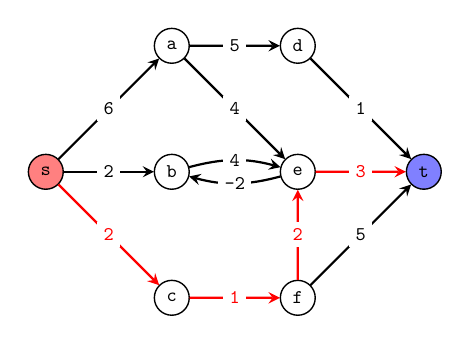
\begin{tikzpicture}[scale=0.8,every node/.style={scale=0.7},font=\tt]
	\SetUpEdge[	lw         = 0.75pt,
				color      = red,
				labelcolor = white]
	\GraphInit[vstyle=Normal] 
	\SetGraphUnit{2}
	\tikzset{VertexStyle/.append  style={fill=red!50}}
	\Vertex{s}
	\tikzset{VertexStyle/.append  style={fill=white}}
	\NOEA(s){a}
	\EA(a){d}
	\tikzset{VertexStyle/.append  style={fill=blue!50}}
	\SOEA(d){t}
	\tikzset{VertexStyle/.append  style={fill=white}}
	\EA(s){b}
	\EA(b){e}
	\SOEA(s){c}
	\EA(c){f}
	\tikzset{EdgeStyle/.style={-stealth, color=black}}
	\Edge[label=6](s)(a)
	\Edge[label=2](s)(b)
	\SetUpEdge[labeltext=red]
	\tikzset{EdgeStyle/.style={-stealth, color=red}}
	\Edge[label=2](s)(c)
	\SetUpEdge[labeltext=black]
	\tikzset{EdgeStyle/.style={-stealth, color=black}}
	\Edge[label=5](a)(d)
	\Edge[label=4](a)(e)
	\tikzset{EdgeStyle/.style={-stealth, color=black, bend left=15}}
	\Edge[label=4](b)(e)
	\Edge[label=-2](e)(b)
	\SetUpEdge[labeltext=red]
	\tikzset{EdgeStyle/.style={-stealth, color=red}}
	\Edge[label=1](c)(f)
	\SetUpEdge[labeltext=black]
	\tikzset{EdgeStyle/.style={-stealth, color=black}}
	\Edge[label=1](d)(t)
	\SetUpEdge[labeltext=red]
	\tikzset{EdgeStyle/.style={-stealth, color=red}}
	\Edge[label=3](e)(t)
	\Edge[label=2](f)(e)
	\SetUpEdge[labeltext=black]
	\tikzset{EdgeStyle/.style={-stealth, color=black}}
	\Edge[label=5](f)(t)
\end{tikzpicture}	
\end{document}
